\chapter{Avaliação e Resultados} \label{chap:resultados}

-Definição da coleção base a analisar

-Definição de quais os conjuntos de teste a criar a partir da coleção base

-Definição das experiências que se pretendem realizar e porquê

-Forma de avaliar e resultados dessas experiências

\section{Coleções de dados} \label{sec:colecoes}

A evolução do estado da arte do reconhecimento facial automático em imagens tem beneficiado em larga escala do aumento constante dos recursos disponíveis para o seu estudo, nomeadamente através da criação de novas e mais completas coleções de dados \cite{Huang2007}. A grande maioria destas coleções, caracteriza-se por ter condições de captura controladas com o intuito de efetuar o estudo de fatores específicos que afetam a qualidade do reconhecimento, tais como a variação da pose, iluminação, expressão e outros fatores mencionados no capítulo \ref{desafios}. O objeto de estudo desta dissertação não é, no entanto, a análise específica de alguns desses fatores, mas sim a criação de um sistema de reconhecimento facial automático em imagens a partir de recursos de código aberto disponíveis, assim como a análise posterior do impacto do uso de abstração de imagens no sistema desenvolvido. Desta forma, a escolha de uma biblioteca apropriada e que represente as grandes variações associadas aos diferentes desafios que afetam o reconhecimento facial em imagens torna-se crucial.

Tendo em conta as preocupações acima mencionadas, para a análise dos resultados obtidos no âmbito nesta dissertação foi escolhida a coleção de imagens \textit{Labeled Faces in the Wild}. Esta coleção é constituída por um conjunto de imagens faciais e respetivas anotações textuais e encontra-se descrita em maior pormenor na secção seguinte deste documento.

Para um estudo científico e rigoroso do desempenho do sistema criado e análise do impacto dos filtros de abstração no reconhecimento facial, para além da escolha de um conjunto de dados a analisar, torna-se também importante a construção de sub-conjuntos de teste, assim como a definição de uma metodologia de avaliação adequada. Na secção \ref{sec:conjuntos} encontram-se detalhados os conjuntos de teste criados e nas secções \ref{falta} e \ref{falta} as metodologias de avaliação adotadas.

\subsection{\textit{Labeled Faces in the Wild}}  \label{sec:lfw}
A coleção \textit{Labeled Faces in the Wild (LFW)} é uma base de dados fotográfica desenhada especificamente para o estudo do problema de reconhecimento facial, particularmente em situações onde as condições de captura das imagens não possuem restrições. Nesse sentido, as imagens que constituem a galeria caracterizam-se por possuir uma grande variabilidade, nomeadamente ao nível da pose, expressão, iluminação, etnia, idade, género, vestuário e qualidade da câmara, por exemplo \cite{Huang2007}.

Nesta coleção encontram-se representados um conjunto de 5749 indivíduos, ilustrados por 13233 imagens. O número de imagens por pessoa apresenta no entanto uma grande variação, desde um mínimo de 1 imagem por pessoa para 4069 indivíduos, até um máximo de 530 imagens que representam o antigo presidente dos Estados Unidos da América George W. Bush. O gráfico \ref{fig:distribuicaoLFW} ilustra a grande variação da distribuição do número de imagens por pessoa.

\begin{figure}[ht]
  \begin{center}
    \leavevmode
    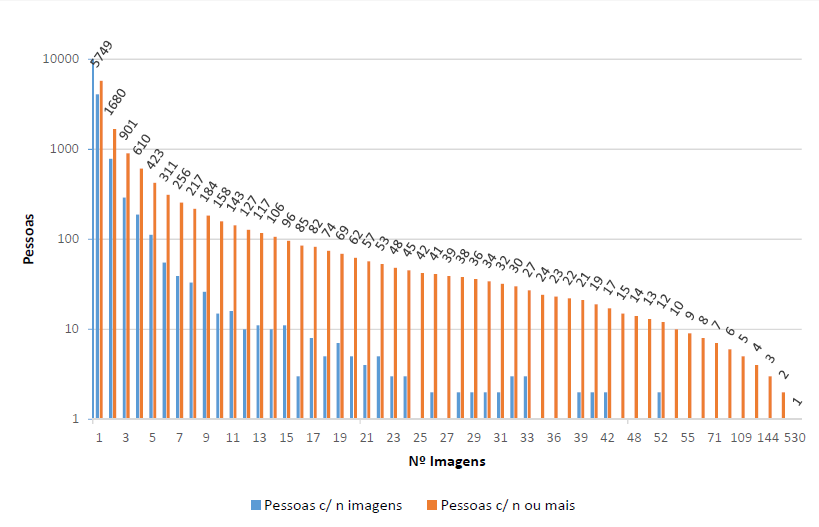
\includegraphics[width=1\textwidth]{Distribuicao}
    \caption{Distribuição do número de imagens por pessoa na biblioteca LFW. No eixo vertical encontram-se representadas o número de pessoas em escala logarítmica e no eixo horizontal o número de imagens correspondente.}
    \label{fig:distribuicaoLFW}
  \end{center}
\end{figure}

Para além da distribuição do número de imagens por pessoa, as restantes características da biblioteca LFW encontram-se resumidas na tabela \ref{tab:lfw}. 
As imagens desta coleção são maioritariamente a cores, com diferentes graus de saturação, existindo também um número reduzido de imagens a preto e branco. Devido à inexistência de restrições na captura de imagens, cada fotografia pode possuir mais do que uma face representada, sendo que a face que contem o pixel central deve ser considerada como a entidade representada na imagem. A cada imagem encontra-se também associada uma anotação textual, relativa ao nome da pessoa representada. A tabela \ref{tab:lfw} sintetiza algumas das características mais significativas da biblioteca.

\begin{center}
\begin{table}
	\caption{Caracterização da Biblioteca LFW}
	\begin{center}
    \begin{tabular}{ll}
    \hline
    Característica                            & Valor            \\ \hline
    Imagens                                   & 13233 imagens    \\
    Pessoas representadas                     & 5749 pessoas     \\
    Tamanho total / Formato                   & 179 MB / JPEG    \\
    Tamanho de cada imagem: min / médio / max & ~                \\
    Dimensões imagem                          & 250 $x$ 250 pixeis \\
    \hline
    \end{tabular}
	\label{tab:lfw}
	\end{center}
\end{table}
\end{center}

Para além da coleção LFW original, encontram-se também disponíveis para fins de investigação duas outras coleções derivadas da coleção original, LFW funneled e LFW-a, onde as imagens originais foram sujeitas a um pré-processamento com vista a efetuar o alinhamento da posição da face na imagem, cada uma correspondendo a uma técnica diferente de alinhamento da imagem, respetivamente. Um exemplo dos resultados obtidos nas diferentes bibliotecas pode ser visto na figura \ref{fig:lfwversoes}.

- figura com três caras cada uma de um LFW diferente.

A coleção LFW é particularmente interessante para o estudo do desempenho do sistema desenvolvido e consequentemente do impacto do uso da abstração de imagens no reconhecimento facial uma vez que a variabilidade presente nas suas imagens, representa uma amostra fiável das variações encontradas no dia-a-dia de uma pessoa. Por outro lado, o facto de as suas imagens não terem sido capturadas com o intuito específico da análise do problema do reconhecimento facial, aproxima este conjunto de dados das imagens utilizadas por um utilizador final de um sistema de reconhecimento facial automático na grande maioria das situações. Finalmente, e uma vez que a tarefa de alinhamento da face na imagem não é um objeto de estudo primordial desta dissertação, a existência de versões já alinhadas da coleção permitiu agilizar os testes realizados, retirando um fator importante de variação dos resultados obtidos. Assim sendo, no âmbito desta dissertação optamos pela utilização da versão alinhada LFW-a \citep{autor} para fins de avaliação do desempenho do sistema de reconhecimento facial criado e do impacto do uso de filtros de abstração sobre essas imagens.

\subsection{Conjuntos de Teste}  \label{sec:conjuntos}
O desempenho de sistemas de reconhecimento facial pode ser analisado através de diferentes perspetivas, tal como introduzido no capítulo \ref{chap:problema} desta dissertação. A biblioteca LFW foi criada com o propósito inicial da análise do sub-problema de reconhecimento facial \textit{pair matching}, no qual o sistema deve decidir se duas faces representam ou não o mesmo indivíduo. No entanto, as características desta biblioteca, nomeadamente no que diz respeito à existência da anotação textual das pessoas presentes em cada imagem, à existência de apenas uma pessoa representada (de forma relevante) em cada imagem e ainda da normalização do formato das imagens, permitem que esta biblioteca possa ser utilizada com um esforço reduzido para o analise dos restantes sub-problemas de reconhecimento facial automático.

No âmbito desta dissertação temos em vista a realização de um conjunto de experiências descritas em \ref{sec:experiencias} e análise dos seus resultados através de duas perspetivas descritas nos pontos \ref{sec:avaliacao1} e \ref{sec:avaliacao2} a seguir. Uma vez que estas avaliações não se encontram enquadradas no paradigma de avaliação de \textit{pair matching}, para o qual a biblioteca LFW foi originalmente criada tornou-se necessário a criação de novos conjuntos de teste. 

Desta forma foram criados 4 conjuntos de teste. Todos os conjuntos possuem um total de 1180 imagens, correspondentes a 59 pessoas diferentes e a 20 imagens por pessoa. Dessas imagens 80"\%" das imagens de cada pessoa são utilizadas como imagens de treino e os restantes 20"\%" como imagens de teste, fazendo assim 16 imagens de treino e 4 de teste por pessoa. A diferença existente entre os diferentes conjuntos está associada às imagens utilizadas como treino e teste do sistema tendo sido criada uma distribuição aleatória para cada um das imagens de cada pessoa para cada um dos conjuntos.

A criação de 4 conjuntos com igual tamanho mas diferentes imagens de treino e teste tem em vista analisar o desempenho do sistema com diferentes galerias de forma a determinar se existe uma variação significativa dos resultados obtidos em cada galeria.

\section{Experiências Realizadas} \label{sec:experiencias}
O módulo de reconhecimento facial, \textit{Face Recognizer}, constituiu uma base sólida para o desenvolvimento do sistema de reconhecimento facial \textit{Visage}. Contudo de modo a tornar o sistema mais completo e versátil revelou-se necessário adaptar o sistema inicialmente existente e expandir as suas capacidades. Esta evolução foi feita de forma gradual e iterativa e culminou num conjunto de experiências que permitem concluir os efeitos das diversas....

O conjunto de imagens que constituem a biblioteca LFW-a foi ainda sujeito a um conjunto de tarefas de pré-processamento com vista a melhorar a eficácia do reconhecimento assim como analisar o impacto dos diferentes pré-processamentos na resolução do problema de reconhecimento facial automático. A cadeia de pré-processamento é constituída por quatro passos, tal como pode ser visualizado na figura \ref{fig:preprocessamento}, sendo que apenas o primeiro é obrigatório para todas as imagens pré-processadas.


\begin{center}
\begin{table}
	\caption{Sub-coleções criadas após pré-processamento.}
	\begin{center}
    \begin{tabular}{lllll}
    \hline\hline
    Designação & Recortada & Normalização           & Filtro Abstração & Máscara \\
        \hline
    Original   & -         & -                      & -                & -       \\
        \hline
    Cropped    & X         & -                      & -                & -       \\
    Masked     & X         & -                      & -                & X       \\
        \hline
    Normalized & X         & Constrast Streching    & -                & X       \\
    Equalized  & X         & Histogram Equalization & -                & X       \\
    CLAHE      & X         & CLAHE                  & -                & X       \\
        \hline
    Bilateral  & X         & Histogram Equalization & Bilateral Filter & X       \\
    Gaussian   & X         & Histogram Equalization & Gaussian Filter  & X       \\
    \hline\hline
    \end{tabular}
	\label{tab:colecoes}
	\end{center}
\end{table}
\end{center}

Da aplicação de diferentes combinações de pré-processamentos aplicados sobre as imagens da coleção LFW-a resultou a criação de um conjunto de novas coleções,  tal como pode ser visualizado na tabela \ref{tab:colecoes}. O primeiro conjunto desta tabela corresponde à coleção original, sobre a qual não foram aplicadas quaisquer tarefas de pré-processamento. Os conjuntos \textit{Masked} e \textit{Cropped}, têm em vista analisar o impacto da remoção de informação redundante que se encontra na imagem, devido à existencia de uma grande àrea de fundo, onde existem, por exemplo, faces de outras pessoas na coleção original. OS conju


\section{Resultados \textit{Closed Set-Identification}} \label{sec:avaliacao1}
Medida padrão de avaliação de reconhecimento facial
Usada em várias avaliações efetuadas, desde a mais antiga FRVT até à recente MBE 2010

\subsection{Metodologias Avaliação}

\subsection{Resultados}

\section{Resultados em Retrieval} \label{sec:avaliacao2}

\subsection{Metodologias Avaliação}

\subsection{Resultados}

